\thispagestyle{empty}
\begin{titlepage}
	\begin{flushleft}
			Bauhaus-Universit�t Weimar\\
			Fakult�t Medien\\
			Studiengang Mediensysteme
	\end{flushleft}
	\begin{verbatim}


	\end{verbatim}
	\begin{center}
		\Large \textbf{Erstellung, Segmentierung und Out-Of-Core-Speichermanagement von Sparse Voxel Octrees}
\begin{figure}[position=h]
  \centering
  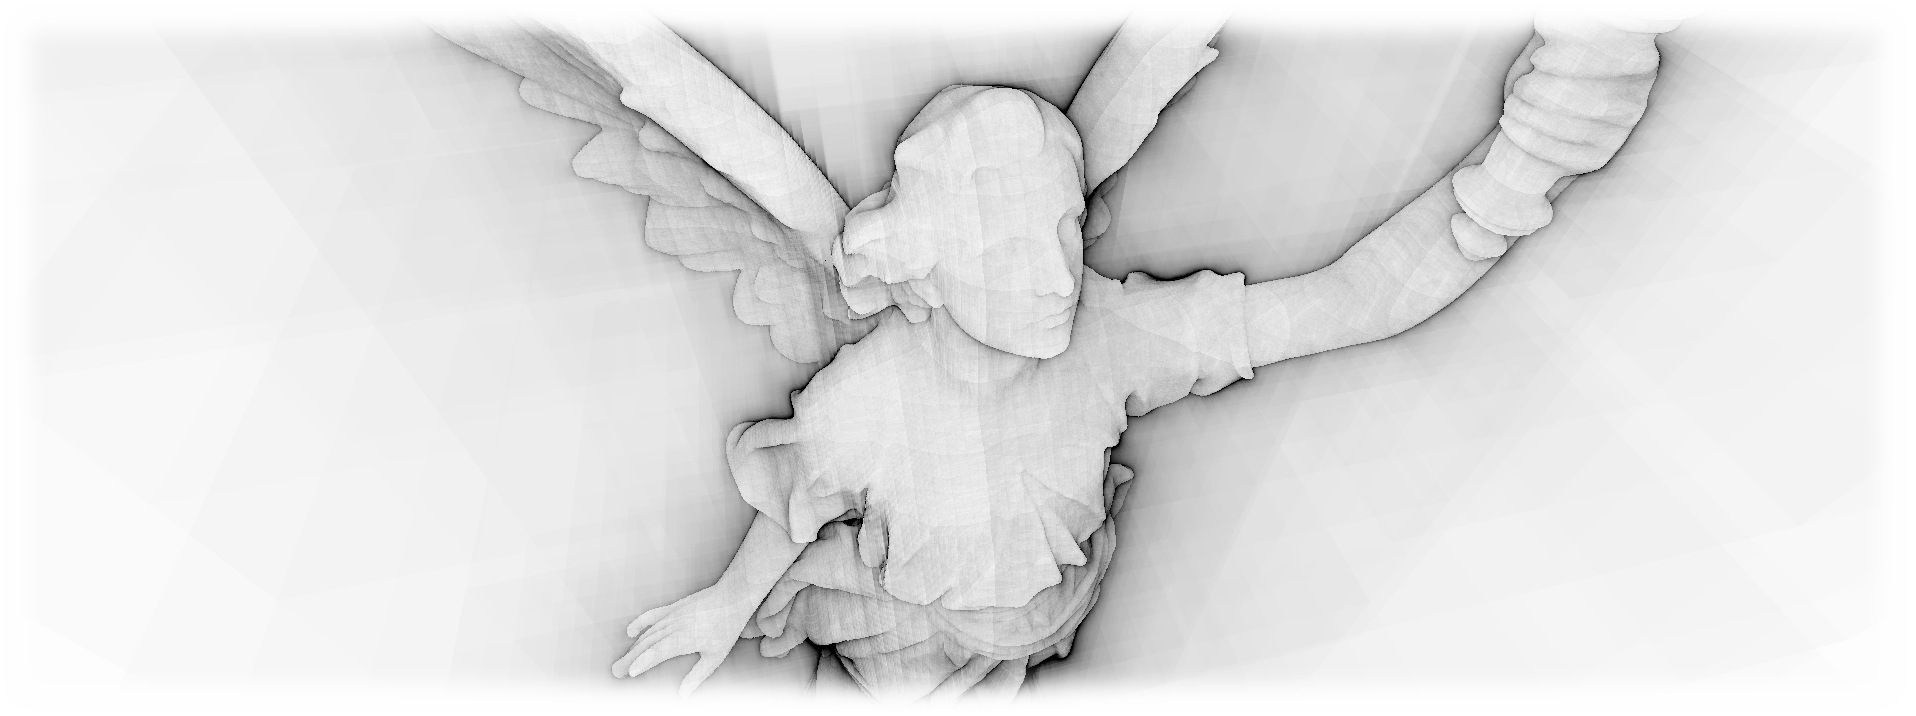
\includegraphics[width=1.0\textwidth]{figures/title_01.png}
\end{figure}

		\Large Diplomarbeit
	\end{center}
	\begin{verbatim}






	\end{verbatim}
	\begin{center}
		Felix Wei�ig\\
		Matrikelnummer: 10596\\
		geb. am 10.10.1979 in Hoyerswerda\\
	\begin{verbatim}


	\end{verbatim}
		1. Gutachter: Prof. Dr. Charles A. W�thrich\\
		2. Gutachter: \_\_\_\_\_\_\_\_\_\_\_\_\_\_\_\_\_\_\_\_\_\_\_ \,\,\,


	\begin{verbatim}

	\end{verbatim}
	Datum der Abgabe: 25. M�rz 2013
	\end{center}

	
\end{titlepage}
